%!TEX root = ../../book_ML.tex
\chapter{Thuật toán học perceptron}
\label{cha:pla}
\index{perceptron}
\index{perceptron learning algorithm}

Cứ làm đi, sai đâu sửa đấy, cuối cùng sẽ thành công! 
 
Đó chính là ý tưởng chính của một thuật toán rất quan trọng trong Machine Learning - thuật toán Perceptron Learning Algorithm hay PLA. 
 
 
 
 
\section{Giới thiệu}
 
Trong bài này, tôi sẽ giới thiệu thuật toán đầu tiên trong Classification có tên là Perceptron Learning Algorithm (PLA) hoặc đôi khi được viết gọn là Perceptron.  
 
Perceptron là một thuật toán Classification cho trường hợp đơn giản nhất: chỉ có hai class (lớp) (\textit{bài toán với chỉ hai class được gọi là binary classification}) và cũng chỉ hoạt động được trong một trường hợp rất cụ thể. Tuy nhiên, nó là nền tảng cho một mảng lớn quan trọng của Machine Learning là Neural Networks và sau này là Deep Learning. (Tại sao lại gọi là Neural Networks - tức mạng dây thần kinh - các bạn sẽ được thấy ở cuối bài). 
 
Giả sử chúng ta có hai tập hợp dữ liệu đã được gán nhãn được minh hoạ trong Hình 1 bên trái dưới đây. Hai class của chúng ta là tập các điểm màu xanh và tập các điểm màu đỏ. Bài toán đặt ra là: từ dữ liệu của hai tập được gán nhãn cho trước, hãy xây dựng một \textit{classifier} (bộ phân lớp) để khi có một điểm dữ liệu hình tam giác màu xám mới, ta có thể dự đoán được màu (nhãn) của nó.  
 
% <table width = "100%" style = "border: 0px solid white"> 
%    <tr > 
%         <td width="40%" style = "border: 0px solid white">  
%         <img style="display:block;" width = "100%" src = "/assets/pla/pla1.png"> 
%          </td> 
%         <td width="40%" style = "border: 0px solid white"> 
%         <img style="display:block;" width = "100%" src = "/assets/pla/pla2.png"> 
%         </td> 
%     </tr> 
% </table>  
% <div class = "thecap">Hình 1: Bài toán Perceptron</div> 

\begin{figure}[t]
     \begin{subfigure}{0.49\textwidth}
     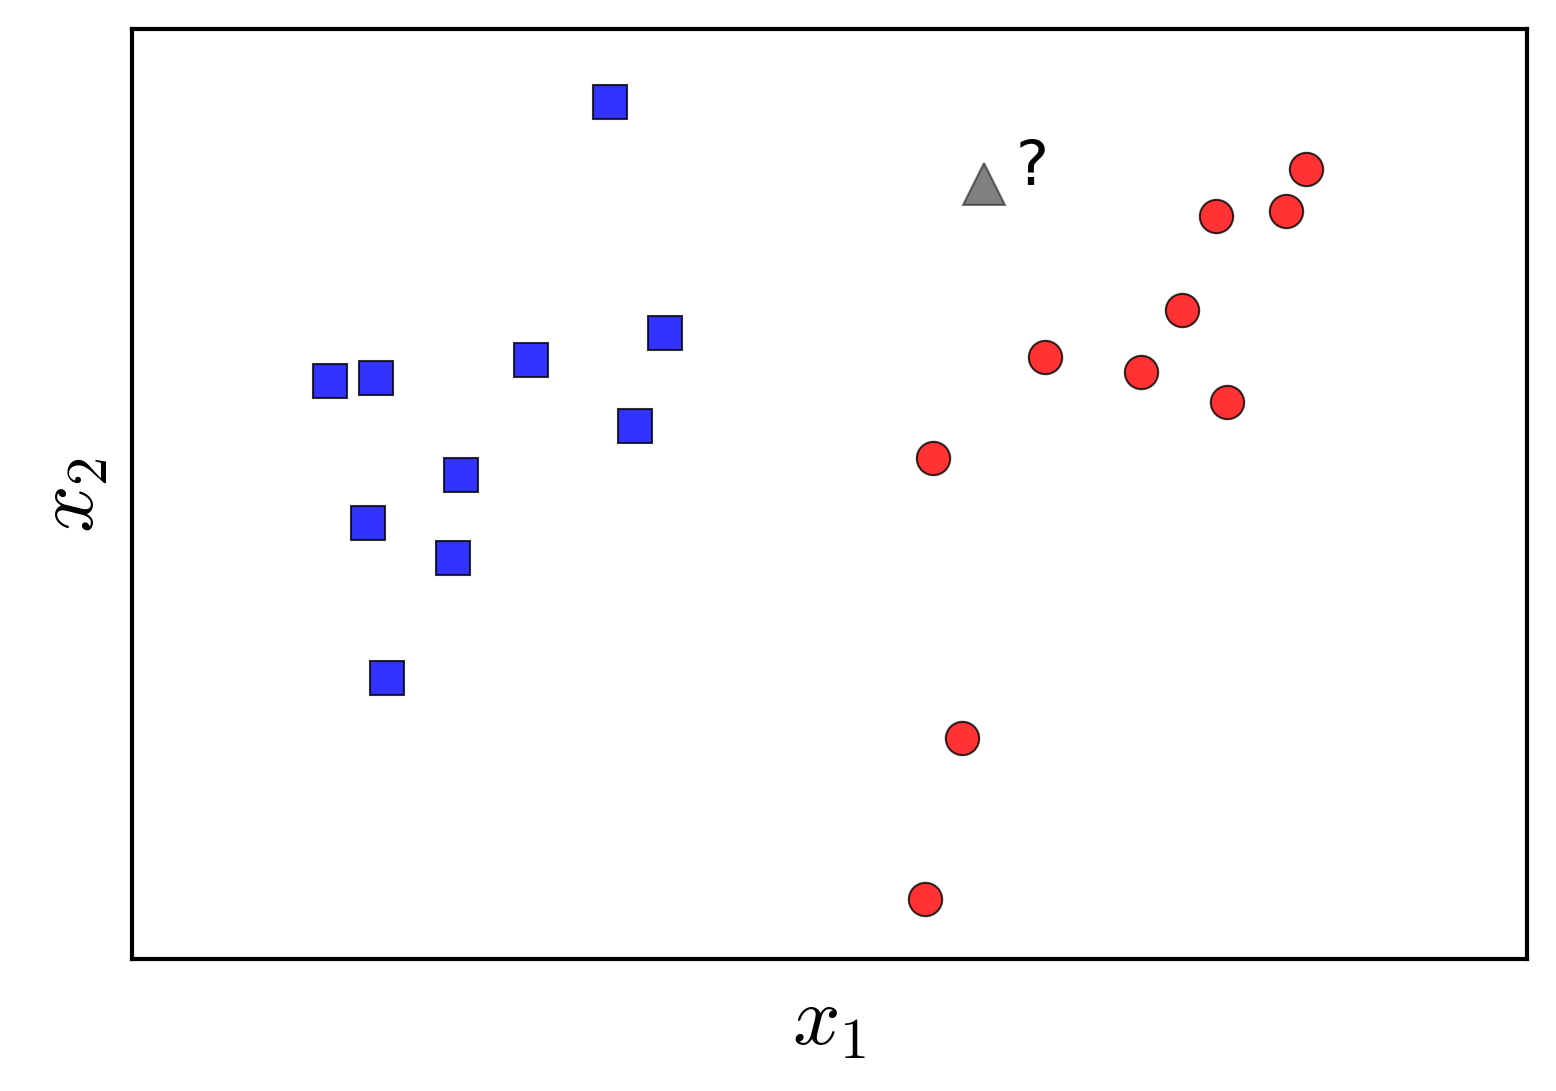
\includegraphics[width=0.99\linewidth]{Chapters/05_NeuralNetworks/09_perceptron/pla1.png}
     \caption{}
     % \label{fig:subim1}
     \end{subfigure}
     \begin{subfigure}{0.49\textwidth}
     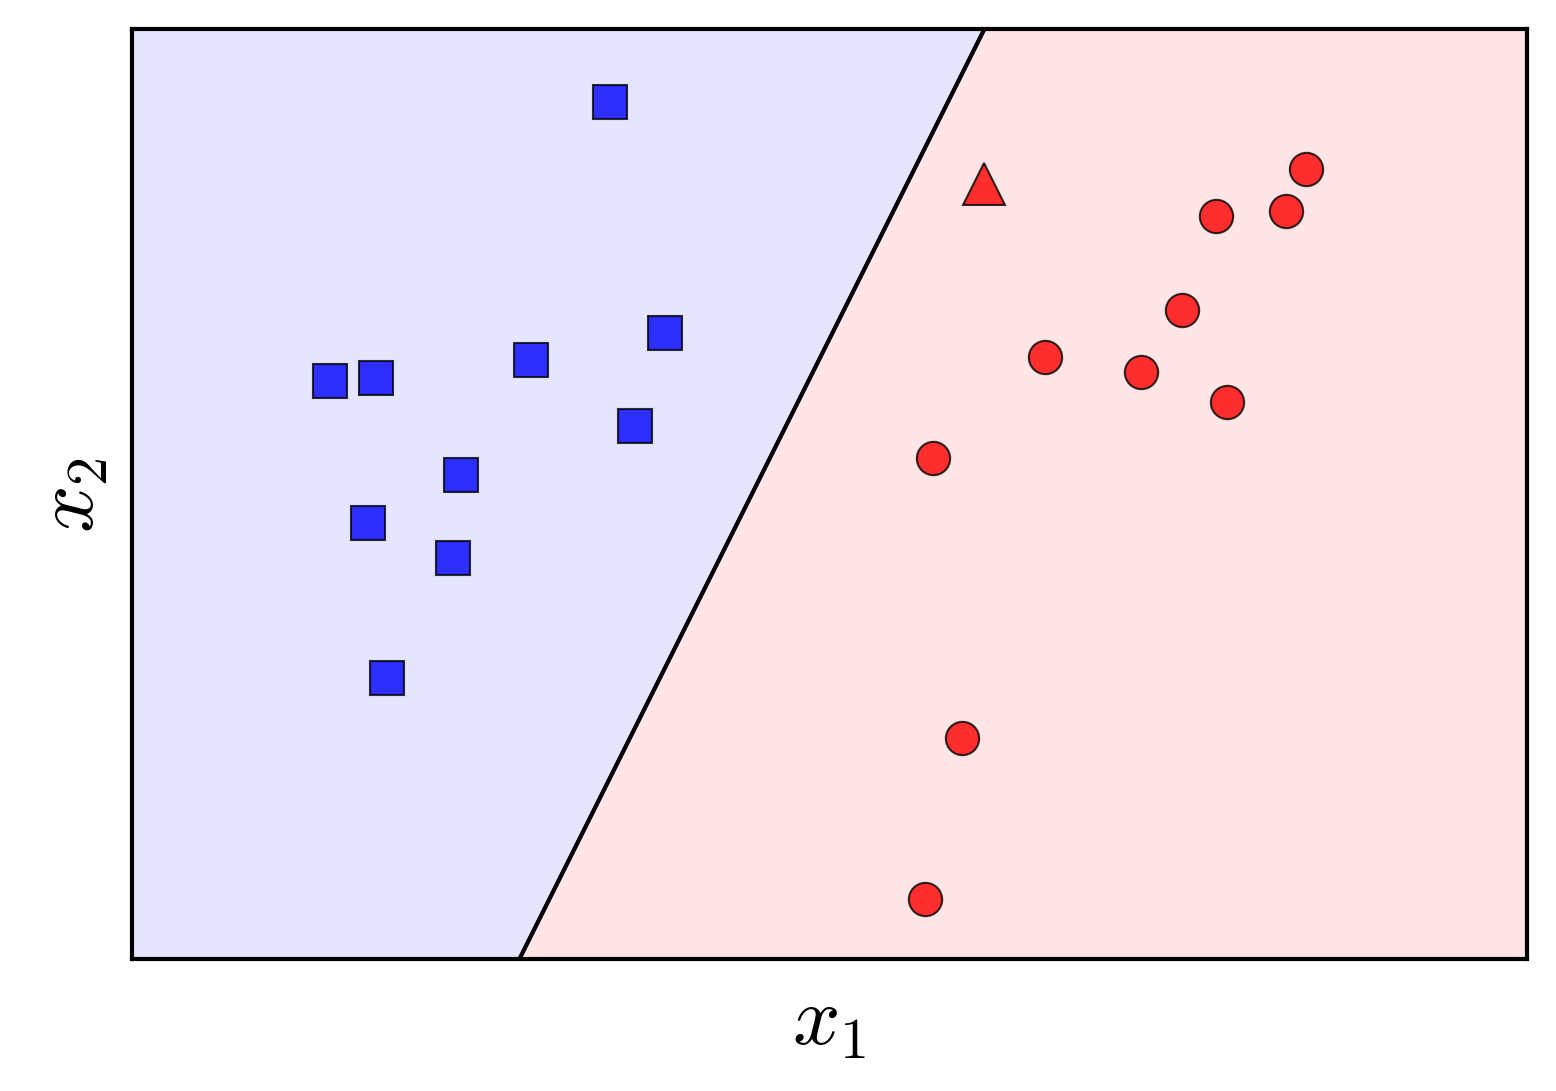
\includegraphics[width=0.99\linewidth]{Chapters/05_NeuralNetworks/09_perceptron/pla2.png}
     \caption{}
     % \label{fig:subim2}
     \end{subfigure}
     \caption{
      Bài toán Perceptron.
     }
     \label{fig:9_1}
 \end{figure}
  

Hiểu theo một cách khác, chúng ta cần tìm \textit{lãnh thổ} của mỗi class sao cho, với mỗi một điểm mới, ta chỉ cần xác định xem nó nằm vào lãnh thổ của class nào rồi quyết định nó thuộc class đó. Để tìm \textit{lãnh thổ} của mỗi class, chúng ta cần đi tìm biên giới (boundary) giữa hai \textit{lãnh thổ} này. Vậy bài toán classification có thể coi là bài toán đi tìm boundary giữa các class. Và boundary đơn giản nhât trong không gian hai chiều là một đường thằng, trong không gian ba chiều là một mặt phẳng, trong không gian nhiều chiều là một siêu mặt phẳng (hyperplane) (tôi gọi chung những boundary này là \textit{đường phẳng}). Những boundary phẳng này được coi là đơn giản vì nó có thể biểu diễn dưới dạng toán học bằng một hàm số đơn giản có dạng tuyến tính, tức linear. Tất nhiên, chúng ta đang giả sử rằng tồn tại một đường phẳng để có thể phân định \textit{lãnh thổ} của hai class. Hình 1 bên phải minh họa một đường thẳng phân chia hai class trong mặt phẳng. Phần có nền màu xanh được coi là \textit{lãnh thổ} của lớp xanh, phần có nên màu đỏ được coi là \textit{lãnh thổ} của lớp đỏ. Trong trường hợp này, điểm dữ liệu mới hình tam giác được phân vào class đỏ.  
 
 
\subsection{Bài toán Perceptron }
Bài toán Perceptron được phát biểu như sau: \textit{Cho hai class được gán nhãn, hãy tìm một đường phẳng sao cho toàn bộ các điểm thuộc class 1 nằm về 1 phía, toàn bộ các điểm thuộc class 2 nằm về phía còn lại của đường phẳng đó. Với giả định rằng tồn tại một đường phẳng như thế.} 
 
Nếu tồn tại một đường phẳng phân chia hai class thì ta gọi hai class đó là \textit{linearly separable}. Các thuật toán classification tạo ra các boundary là các đường phẳng được gọi chung là Linear Classifier. 
 
 
\section{Thuật toán Perceptron (PLA)}
Cũng giống như các thuật toán lặp trong \href{http://machinelearningcoban.com/2017/01/01/kmeans/}{K-means Clustering} và \href{http://machinelearningcoban.com/2017/01/12/gradientdescent/}{Gradient Descent}, ý tưởng cơ bản của PLA là xuất phát từ một nghiệm dự đoán nào đó, qua mỗi vòng lặp, nghiệm sẽ được cập nhật tới một ví trí tốt hơn. Việc cập nhật này dựa trên việc giảm giá trị của một hàm mất mát nào đó.  
 
 
\subsection{Một số ký hiệu}
Giả sử $\mathbf{X} = [\mathbf{x}_1, \mathbf{x}_2, \dots, \mathbf{x}_N] \in \mathbb{R}^{d \times N}$ là ma trận chứa các điểm dữ liệu mà mỗi cột $\mathbf{x}_i \in \mathbb{R}^{d\times 1}$ là một điểm dữ liệu trong không gian $d$ chiều. (\textit{Chú ý: khác với các bài trước tôi thường dùng các vector hàng để mô tả dữ liệu, trong bài này tôi dùng vector cột để biểu diễn. Việc biểu diễn dữ liệu ở dạng hàng hay cột tùy thuộc vào từng bài toán, miễn sao cách biễu diễn toán học của nó khiến cho người đọc thấy dễ hiểu}). 
 
Giả sử thêm các nhãn tương ứng với từng điểm dữ liệu được lưu trong một vector hàng $\mathbf{y} = [y_1, y_2, \dots, y_N] \in \mathbb{R}^{1\times N}$, với $y_i = 1$ nếu $\mathbf{x}_i$ thuộc class 1 (xanh) và $y_i = -1$ nếu $\mathbf{x}_i$ thuộc class 2 (đỏ). 
 
Tại một thời điểm, giả sử ta tìm được boundary là đường phẳng có phương trình: 
\begin{eqnarray} 
    f_{\mathbf{w}}(\mathbf{x}) &=& w_1x_1 + \dots + w_dx_d + w_0 \\\  
    &=&\mathbf{w}^T\mathbf{\bar{x}} = 0 
\end{eqnarray} 
 
với $\mathbf{\bar{x}}$ là điểm dữ liệu mở rộng bằng cách thêm phần tử $x_0 = 1$ lên trước vector $\mathbf{x}$ tương tự như trong \href{http://machinelearningcoban.com/2016/12/28/linearregression/}{Linear Regression}. Và từ đây, khi nói $\mathbf{x}$, tôi cũng ngầm hiểu là điểm dữ liệu mở rộng. 
 
Để cho đơn giản, chúng ta hãy cùng làm việc với trường hợp mỗi điểm dữ liệu có số chiều $d = 2$. Giả sử đường thẳng $w_1 x_1 + w_2 x_2 + w_0 = 0$ chính là nghiệm cần tìm như Hình 2 dưới đây: 
 
% <div class="imgcap"> 
% <img src ="\assets\pla\pla4.png" align = "center" width = "400"> 
% <div class = "thecap">Hình 2: Phương trình đường thẳng boundary.</div> 
% </div> 

\begin{figure}[t]
     % caption on side     
     \floatbox[{\capbeside\thisfloatsetup{capbesideposition={right,top},capbesidewidth=6cm}}]{figure}[\FBwidth]
     {\caption{ 
     Phương trình đường thẳng phân chia hai lớp.
     }
     \label{fig:9_2}}
     { % figure here
     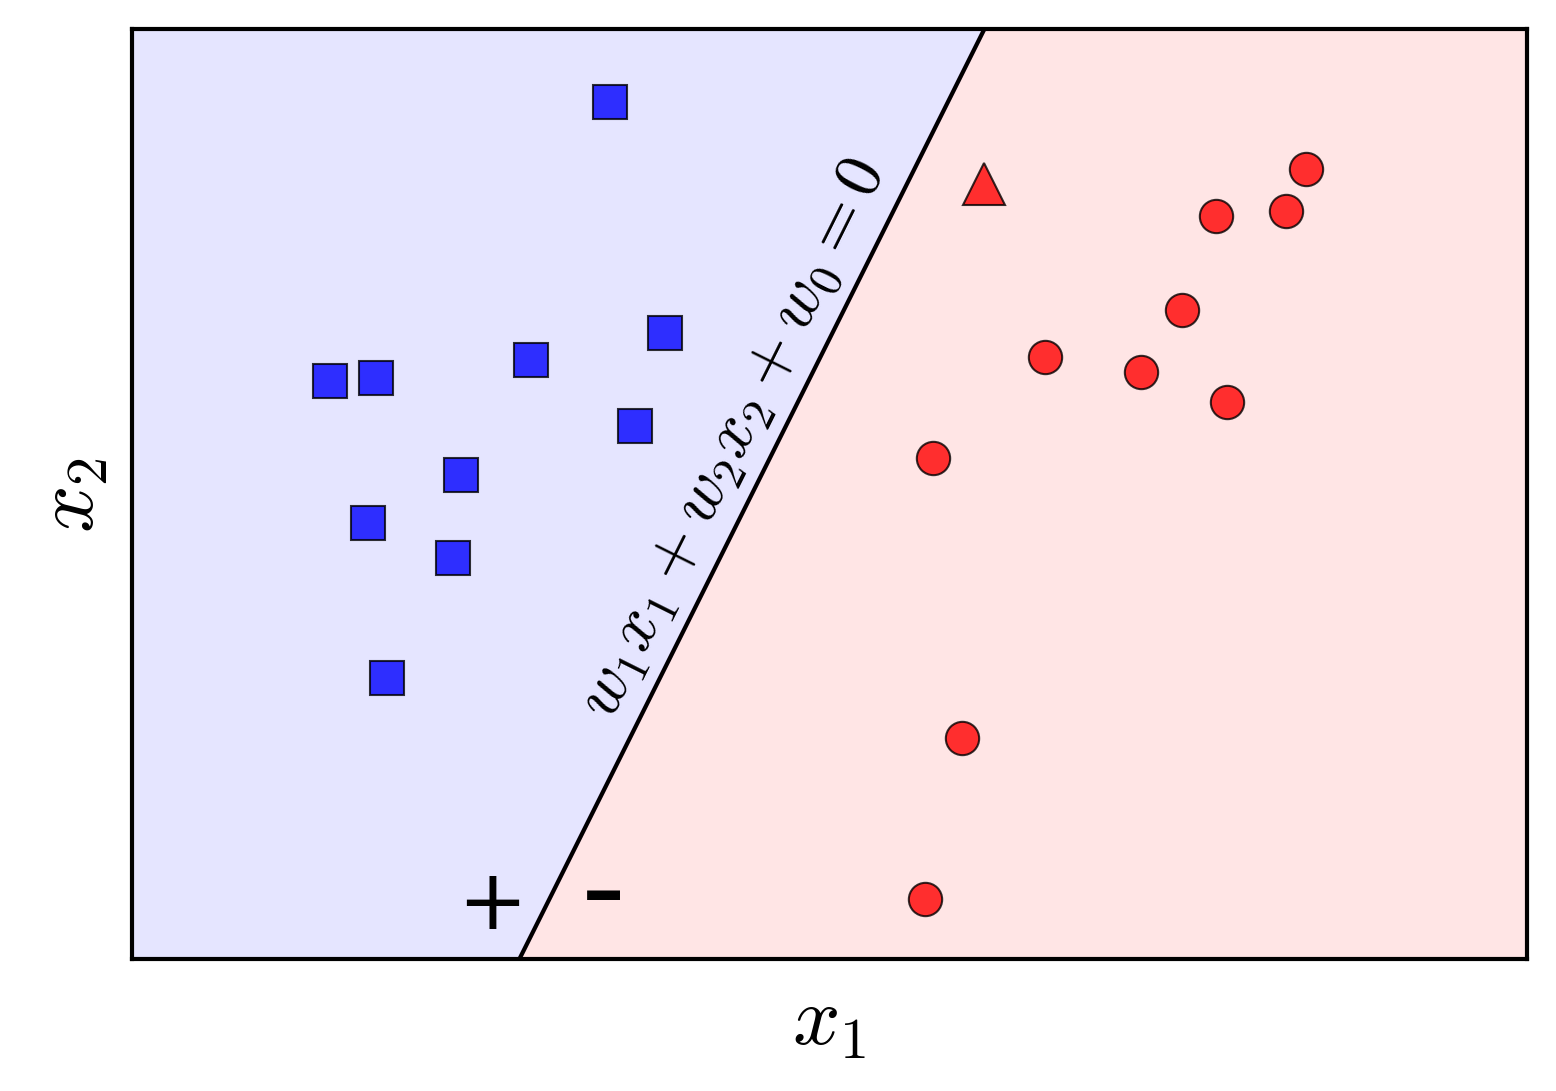
\includegraphics[width=.5\textwidth]{Chapters/05_NeuralNetworks/09_perceptron/pla4.png}
     }
 \end{figure}

 
Nhận xét rằng các điểm nằm về cùng 1 phía so với đường thẳng này sẽ làm cho hàm số $f_{\mathbf{w}}(\mathbf{x})$ mang cùng dấu. Chỉ cần đổi dấu của $\mathbf{w}$ nếu cần thiết, ta có thể giả sử các điểm nằm trong nửa mặt phẳng nền xanh mang dấu dương (+), các điểm nằm trong nửa mặt phẳng nền đỏ mang dấu âm (-). Các dấu này cũng tương đương với nhãn $y$ của mỗi class. Vậy nếu $\mathbf{w}$ là một nghiệm của bài toán Perceptron, với một điểm dữ liệu mới $\mathbf{x}$ chưa được gán nhãn, ta có thể xác định class của nó bằng phép toán đơn giản như sau: 
\begin{equation} 
\text{label}(\mathbf{x}) = 1 ~\text{if}~ \mathbf{w}^T\mathbf{x} \geq 0, \text{otherwise} -1 
\end{equation} 
 
Ngắn gọn hơn:  
\begin{equation} 
    \text{label}(\mathbf{x}) = \text{sgn}(\mathbf{w}^T\mathbf{x}) 
\end{equation} 
trong đó, $\text{sgn}$ là hàm xác định dấu, với giả sử rằng $\text{sgn}(0) = 1$. 
 
 
\subsection{Xây dựng hàm mất mát}
Tiếp theo, chúng ta cần xây dựng hàm mất mát với tham số $\mathbf{w}$ bất kỳ. Vẫn trong không gian hai chiều, giả sử đường thẳng $w_1x_1 + w_2x_2 + w_0 = 0$ được cho như Hình 3 dưới đây: 
% <div class="imgcap"> 
% <img src ="\assets\pla\pla3.png" align = "center" width = "400"> 
% <div class = "thecap">Hình 3: Đường thẳng bất kỳ và các điểm bị misclassified được khoanh tròn.</div> 
% </div>  

\begin{figure}[t]
    % caption on side     
    \floatbox[{\capbeside\thisfloatsetup{capbesideposition={right,top},capbesidewidth=6cm}}]{figure}[\FBwidth]
    {\caption{ 
    Ví dụ về một đường thẳng bất kỳ và các điểm bị misclassified được khoanh tròn.
    }
    \label{fig:9_3}}
    { % figure here
    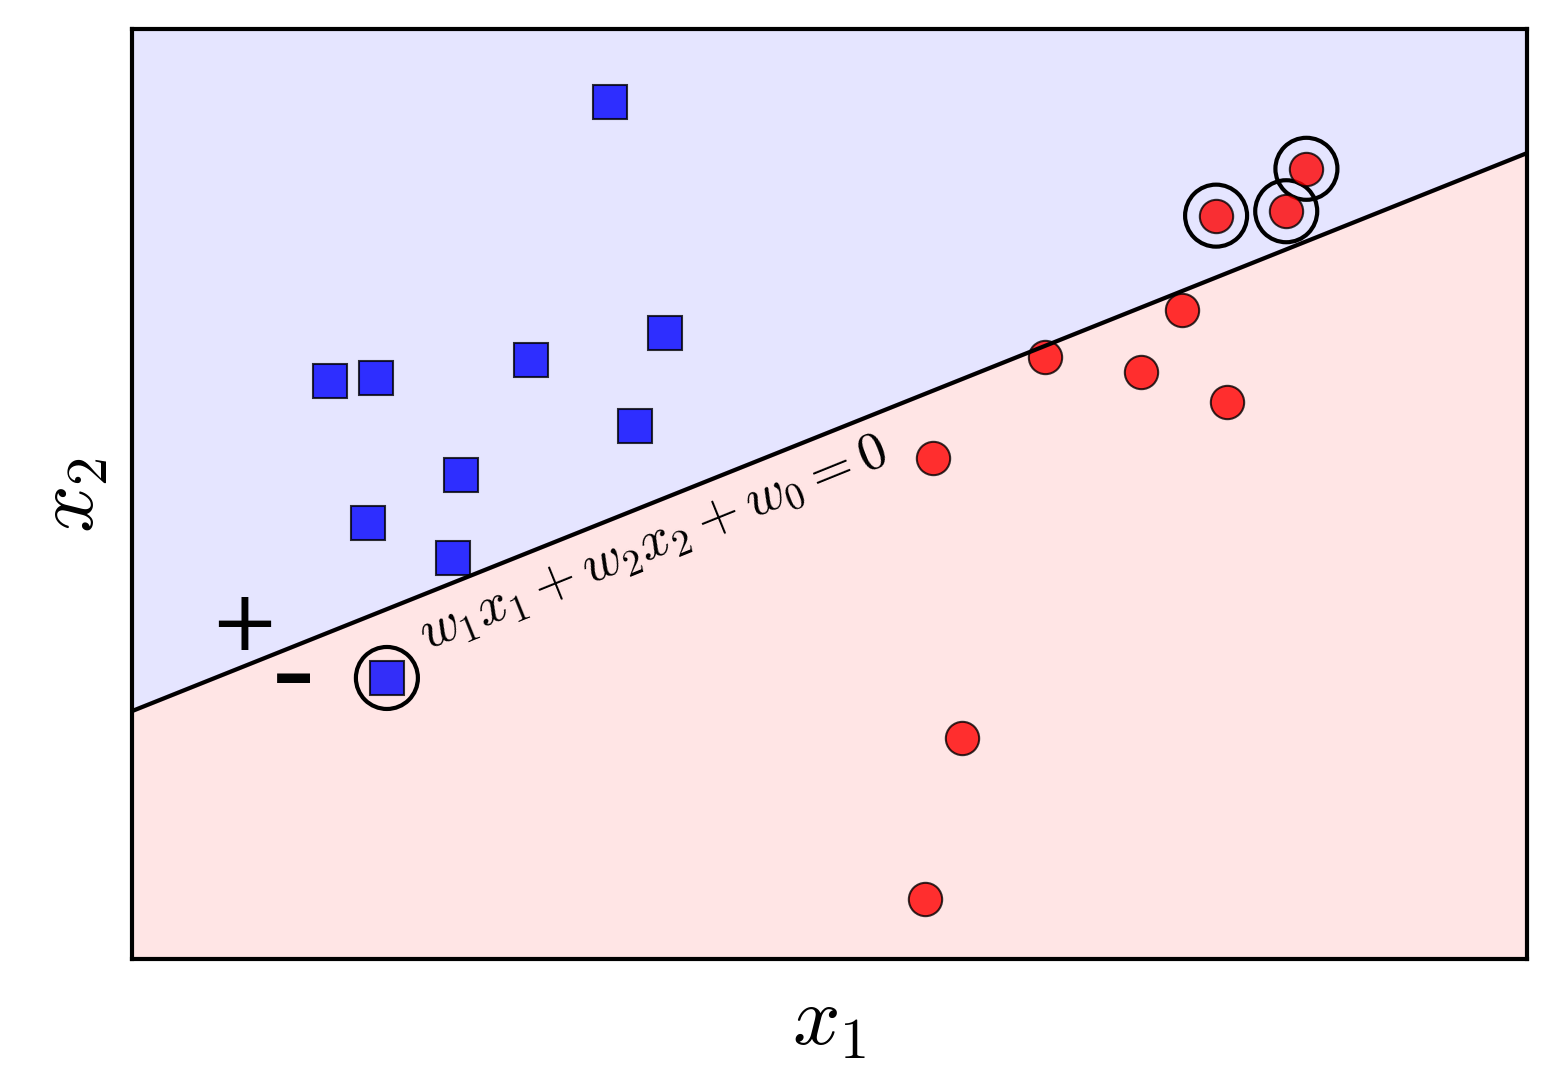
\includegraphics[width=.5\textwidth]{Chapters/05_NeuralNetworks/09_perceptron/pla3.png}
    }
\end{figure}

 
Trong trường hợp này, các điểm được khoanh tròn là các điểm bị misclassified (phân lớp lỗi). Điều chúng ta mong muốn là không có điểm nào bị misclassified. Hàm mất mát đơn giản nhất chúng ta nghĩ đến là hàm \textit{đếm} số lượng các điểm bị misclassied và tìm cách tối thiểu hàm số này: 
\begin{equation} 
    J_1(\mathbf{w}) = \sum_{\mathbf{x}_i \in \mathcal{M}} (-y_i\text{sgn}(\mathbf{w}^T\mathbf{x_i})) 
\end{equation} 
 
trong đó $\mathcal{M}$ là tập hợp các điểm bị misclassifed (\textit{tập hợp này thay đổi theo} $\mathbf{w}$). Với mỗi điểm $\mathbf{x}_i \in \mathcal{M}$, vì điểm này bị misclassified nên $y_i$ và $\text{sgn}(\mathbf{w}^T\mathbf{x})$ khác nhau, và vì thế $-y_i\text{sgn}(\mathbf{w}^T\mathbf{x_i}) = 1 $. Vậy $J_1(\mathbf{w})$ chính là hàm \textit{đếm} số lượng các điểm bị misclassified. Khi hàm số này đạt giá trị nhỏ nhất bằng 0 thì ta không còn điểm nào bị misclassified.  
 
Một điểm quan trọng, hàm số này là rời rạc, không tính được đạo hàm theo $\mathbf{w}$ nên rất khó tối ưu. Chúng ta cần tìm một hàm mất mát khác để việc tối ưu khả thi hơn. 
 
Xét hàm mất mát sau đây:  
 
\begin{equation} 
    J(\mathbf{w}) = \sum_{\mathbf{x}_i \in \mathcal{M}} (-y_i\mathbf{w}^T\mathbf{x_i}) 
\end{equation} 
 
Hàm $J()$ khác một chút với hàm $J_1()$ ở việc bỏ đi hàm $\text{sgn}$. Nhận xét rằng khi một điểm misclassified $\mathbf{x}_i$ nằm càng xa boundary thì giá trị $-y_i\mathbf{w}^T\mathbf{x}_i$ sẽ càng lớn, nghĩa là sự sai lệch càng lớn. Giá trị nhỏ nhất của hàm mất mát này cũng bằng 0 nếu không có điểm nào bị misclassifed. Hàm mất mát này cũng được cho là tốt hơn hàm $J_1()$ vì nó \textit{trừng phạt} rất nặng những điểm \textit{lấn sâu sang lãnh thổ của class kia}. Trong khi đó, $J_1()$ \textit{trừng phạt} các điểm misclassified như nhau (đều = 1), bất kể chúng xa hay gần với đường biên giới. 
 
Tại một thời điểm, nếu chúng ta chỉ quan tâm tới các điểm bị misclassified thì hàm số $J(\mathbf{w})$ khả vi (tính được đạo hàm), vậy chúng ta có thể sử dụng \href{http://machinelearningcoban.com/2017/01/12/gradientdescent/}{Gradient Descent} hoặc \href{http://machinelearningcoban.com/2017/01/16/gradientdescent2/#-stochastic-gradient-descent}{Stochastic Gradient Descent (SGD)} để tối ưu hàm mất mát này. Với ưu điểm của SGD cho các bài toán \href{http://machinelearningcoban.com/2017/01/12/gradientdescent/#large-scale}{large-scale}, chúng ta sẽ làm theo thuật toán này.  
 
Với \textit{một} điểm dữ liệu $\mathbf{x}_i$ bị misclassified, hàm mất mát trở thành: 
 
\begin{equation} 
    J(\mathbf{w}; \mathbf{x}_i; y_i) = -y_i\mathbf{w}^T\mathbf{x}_i 
\end{equation} 
 
Đạo hàm tương ứng: 
 
\begin{equation} 
    \nabla_{\mathbf{w}}J(\mathbf{w}; \mathbf{x}_i; y_i) = -y_i\mathbf{x}_i 
\end{equation} 
Vậy quy tắc cập nhật là: 
\begin{equation} 
\mathbf{w} = \mathbf{w} + \eta y_i\mathbf{x}_i 
\end{equation} 
với $\eta$ là learning rate.  
 
Nhận xét rằng nếu $\mathbf{w}$ là nghiệm thì $\eta\mathbf{w}$ cũng là nghiệm với $\eta$ là một số khác 0 bất kỳ. Vậy nếu $\mathbf{w}_0$ nhỏ gần với 0 và số vòng lặp đủ lớn, ta có thể coi như learning rate $\eta = 1$. Ta có một quy tắc cập nhật rất gọn là: $\mathbf{w}_{t+1} = \mathbf{w}_{t} + y_i\mathbf{x}_i$. Nói cách khác, với mỗi điểm $\mathbf{x}_i$ bị misclassifed, ta chỉ cần nhân điểm đó với nhãn $y_i$ của nó, lấy kết quả cộng vào $\mathbf{w}$ ta sẽ được $\mathbf{w}$ mới. 
 
Ta có một quan sát nhỏ ở đây: 
\begin{equation} 
\mathbf{w}_{t+1}^T\mathbf{x}_i = (\mathbf{w}_{t} + y_i\mathbf{x}_i)^T\mathbf{x}_{i} \\\ 
= \mathbf{w}_{t}^T\mathbf{x}_i + y_i \|\mathbf{x}_i\|_2^2 
\end{equation} 
 
Nếu $y_i = 1$, vì $\mathbf{x}_i$ bị misclassifed nên $\mathbf{w}_{t}^T\mathbf{x}_i < 0$. Cũng vì $y_i = 1$ nên $y_i \|\mathbf{x}_i\|_2^2 = \|\mathbf{x}_i\|_2^2 \geq 1$ (chú ý $x_0 = 1$), nghĩa là $\mathbf{w}_{t+1}^T\mathbf{x}_i > \mathbf{w}_{t}^T\mathbf{x}_i$. Lý giải bằng lời, $\mathbf{w}_{t+1}$ tiến về phía làm cho $\mathbf{x}_i$ được phân lớp đúng. Điều tương tự xảy ra nếu $y_i = -1$. 
 
Đến đây, cảm nhận của chúng ta với thuật toán này là: cứ chọn đường boundary đi. Xét từng điểm một, nếu điểm đó bị misclassified thì tiến đường boundary về phía làm cho điểm đó được classifed đúng. Có thể thấy rằng, khi di chuyển đường boundary này, các điểm trước đó được classified đúng có thể lại bị misclassified. Mặc dù vậy, PLA vẫn được đảm bảo sẽ hội tụ sau một số hữu hạn bước (tôi sẽ chứng minh việc này ở phía sau của bài viết). Tức là cuối cùng, ta sẽ tìm được đường phẳng phân chia hai lớp, miễn là hai lớp đó là linearly separable. Đây cũng chính là lý do câu đầu tiên trong bài này tôi nói với các bạn là: "Cứ làm đi, sai đâu sửa đấy, cuối cùng sẽ thành công!". 
 
Tóm lại, thuật toán Perceptron có thể được viết như sau: 
 
 
\subsection{Tóm tắt PLA }
\begin{enumerate}
\item Chọn ngẫu nhiên một vector hệ số $\mathbf{w}$ với các phần tử gần 0. 
\item Duyệt ngẫu nhiên qua từng điểm dữ liệu $\mathbf{x}_i$: 
    \item Nếu $\mathbf{x}_i$ được phân lớp đúng, tức $\text{sgn}(\mathbf{w}^T\mathbf{x}_i) = y_i$, chúng ta không cần làm gì. 
    \item Nếu $\mathbf{x}_i$ bị misclassifed, cập nhật $\mathbf{w}$ theo công thức: 
    \begin{equation} 
    \mathbf{w} = \mathbf{w} + y_i\mathbf{x}_i 
    \end{equation} 
\item Kiểm tra xem có bao nhiêu điểm bị misclassifed. Nếu không còn điểm nào, dừng thuật toán. Nếu còn, quay lại bước 2. 
\end{enumerate}
 
 
 
 
\section{Ví dụ trên Python}
Như thường lệ, chúng ta sẽ thử một ví dụ nhỏ với Python. 
 
 
\subsection{Load thư viện và tạo dữ liệu}
Chúng ta sẽ tạo hai nhóm dữ liệu, mỗi nhóm có 10 điểm, mỗi điểm dữ liệu có hai chiều để thuận tiện cho việc minh họa. Sau đó, tạo dữ liệu mở rộng bằng cách thêm 1 vào đầu mỗi điểm dữ liệu.  
 
 
\begin{lstlisting}[language=Python]
# generate data 
# list of points  
import numpy as np  
import matplotlib.pyplot as plt 
from scipy.spatial.distance import cdist 
np.random.seed(2) 
 
means = [[2, 2], [4, 2]] 
cov = [[.3, .2], [.2, .3]] 
N = 10 
X0 = np.random.multivariate_normal(means[0], cov, N).T 
X1 = np.random.multivariate_normal(means[1], cov, N).T 
 
X = np.concatenate((X0, X1), axis = 1) 
y = np.concatenate((np.ones((1, N)), -1*np.ones((1, N))), axis = 1) 
# Xbar  
X = np.concatenate((np.ones((1, 2*N)), X), axis = 0) 
\end{lstlisting}
 
Sau khi thực hiện đoạn code này, biến \pythoninline{X} sẽ chứa dữ liệu input (mở rộng), biến \pythoninline{y} sẽ chứa nhãn của mỗi điểm dữ liệu trong \pythoninline{X}. 
 
\subsection{Các hàm số cho PLA}
Tiếp theo chúng ta cần viết 3 hàm số cho PLA: 
\begin{enumerate}
    \item \pythoninline{h(w, x)}: tính đầu ra khi biết đầu vào \pythoninline{x} và weights \pythoninline{w}.
    \item \pythoninline{has_converged(X, y, w)}: kiểm tra xem thuật toán đã hội tụ chưa. Ta chỉ cần so sánh \pythoninline{h(w, X)} với \textit{ground truth} \pythoninline{y}. Nếu giống nhau thì dừng thuật toán. 
    \item \pythoninline{perceptron(X, y, w_init)}: hàm chính thực hiện PLA. 
\end{enumerate}
 
\begin{lstlisting}[language=Python]
def h(w, x):     
    return np.sign(np.dot(w.T, x)) 
 
def has_converged(X, y, w):     
    return np.array_equal(h(w, X), y)  
 
def perceptron(X, y, w_init): 
    w = [w_init] 
    N = X.shape[1] 
    d = X.shape[0] 
    mis_points = [] 
    while True: 
        # mix data  
        mix_id = np.random.permutation(N) 
        for i in range(N): 
            xi = X[:, mix_id[i]].reshape(d, 1) 
            yi = y[0, mix_id[i]] 
            if h(w[-1], xi)[0] != yi: # misclassified point 
                mis_points.append(mix_id[i]) 
                w_new = w[-1] + yi*xi  
                w.append(w_new) 
                 
        if has_converged(X, y, w[-1]): 
            break 
    return (w, mis_points) 
 
d = X.shape[0] 
w_init = np.random.randn(d, 1) 
(w, m) = perceptron(X, y, w_init) 
\end{lstlisting}
 
Dưới đây là hình minh họa thuật toán PLA cho bài toán nhỏ này: 
 
% <div class="imgcap"> 
% <img src ="\assets\pla\pla_vis.gif" align = "center" width = "400"> 
% <div class = "thecap"> Hình 4: Minh họa thuật toán PLA </div> 
% </div>  

{\color{red} GIF IMAGES}

Sau khi cập nhật 18 lần, PLA đã hội tụ. Điểm được khoanh tròn màu đen là điểm misclassified tương ứng được chọn để cập nhật đường boundary.  
 
Source code cho phần này (bao gồm hình động) \href{https://github.com/tiepvupsu/tiepvupsu.github.io/blob/master/assets/pla/perceptron.py}{có thể được tìm thấy ở đây}. 
 
 
\section{Chứng minh hội tụ}
 
Giả sử rằng $\mathbf{w}^*$ là một nghiệm của bài toán (ta có thể giả sử việc này được vì chúng ta đã có giả thiết hai class là linearly separable - tức tồn tại nghiệm). Có thể thấy rằng, với mọi $\alpha > 0$, nếu $\mathbf{w}^*$ là nghiệm, $\alpha\mathbf{w}^*$ cũng là nghiệm của bài toán. Xét dãy số không âm $ u_{\alpha}(t) = \|\mathbf{w}_{t} - \alpha\mathbf{w}^*\|_2^2$. Với $\mathbf{x}_i$ là một điểm bị misclassified nếu dùng nghiệm $\mathbf{w}_t$ ta có:  
 
 
 
 
\begin{eqnarray} 
    &&u_{\alpha}(t+1) = \|\mathbf{w}_{t+1} - \alpha \mathbf{w}^*\|_2^2 \\\ 
    &=& \|\mathbf{w}_{t} + y_i\mathbf{x}_i - \alpha\mathbf{w}^*\|_2^2 \\\ 
    &=& \|\mathbf{w}_{t} -\alpha\mathbf{w}^*\|_2^2 + y_i^2\|\mathbf{x}_i\|_2^2 + 2y_i\mathbf{x}_i^T(\mathbf{w} - \alpha\mathbf{w}^*) \\\ 
    &<& u_{\alpha}(t) \ + \|\mathbf{x}_i\|_2^2 - 2\alpha y_i\mathbf{x}_i^T \mathbf{w}^* 
\end{eqnarray} 
 
 
Dấu nhỏ hơn ở dòng cuối là vì $y_i^2 = 1$ và $2y_i\mathbf{x}_i^T\mathbf{w}_{t} < 0$. Nếu ta đặt:  
 
\begin{eqnarray} 
\beta^2 &=& \max_{i=1, 2, \dots, N}\|\mathbf{x}_i\|_2^2 \\\ 
\gamma &=& \min_{i=1, 2, \dots, N} y_i\mathbf{x}_i^T\mathbf{w}^\} 
\end{eqnarray} 
 
và chọn $\alpha = \frac{\beta^2}{\gamma}$, ta có: 
\begin{equation} 
0 \leq u_{\alpha}(t+1) < u_{\alpha}(t) + \beta^2 - 2\alpha\gamma = u_{\alpha}(t) - \beta^2 
\end{equation} 
 
Điều này nghĩa là: nếu luôn luôn có các điểm bị misclassified thì dãy $u_{\alpha}(t)$ là dãy giảm, bị chặn dưới bởi 0, và phần tử sau kém phần tử trước ít nhất một lượng là $\beta^2>0$. Điều vô lý này chứng tỏ đến một lúc nào đó sẽ không còn điểm nào bị misclassified. Nói cách khác, thuật toán PLA hội tụ sau một số hữu hạn bước.  
 
 
\section{Mô hình Neural Network đầu tiên}
Hàm số xác định class của Perceptron $\text{label}(\mathbf{x}) = \text{sgn}(\mathbf{w}^T\mathbf{x})$ có thể được mô tả như hình vẽ (được gọi là network) dưới đây: 
 
% <div class="imgcap"> 
% <img src ="\assets\pla\pla_nn.png" align = "center" width = "800"> 
% <div class = "thecap"> Hình 5: Biểu diễn của Perceptron dưới dạng Neural Network.</div> 
% </div>  
\begin{figure}[t]
     % caption on side     
     \floatbox[{\capbeside\thisfloatsetup{capbesideposition={right,top},capbesidewidth=6cm}}]{figure}[\FBwidth]
     {\caption{ 
     Biểu diễn của Perceptron dưới dạng Neural Network.
     }
     \label{fig:9_5}}
     { % figure here
     \includegraphics[width=.5\textwidth]{Chapters/05_NeuralNetworks/09_perceptron/latex/pla_nn.pdf}
     }
 \end{figure}
  
Đầu vào của network $\mathbf{x}$ được minh họa bằng các node màu xanh lục với node $x_0$ luôn luôn bằng 1. Tập hợp các node màu xanh lục được gọi là \textit{Input layer}. Trong ví dụ này, tôi giả sử số chiều của dữ liệu $d = 4$. Số node trong input layer luôn luôn là $d + 1$ với một node là 1 được thêm vào. Node $x_0 = 1$ này đôi khi được ẩn đi.  
 
Các trọng số (\textit{weights}) $w_0, w_1, \dots, w_d$ được gán vào các mũi tên đi tới node $\displaystyle z = \sum_{i=0}^dw_ix_i = \mathbf{w}^T\mathbf{x}$. Node $y = \text{sgn}(z)$ là \textit{output} của network. Ký hiệu hình chữ Z ngược màu xanh trong node $y$ thể hiện đồ thị của hàm số $\text{sgn}$.  
 
Trong thuật toán PLA, ta phải tìm các weights trên các mũi tên sao cho với mỗi $\mathbf{x}_i$ ở tập các điểm dữ liệu đã biết được đặt ở Input layer, output của network này trùng với nhãn $y_i$ tương ứng.  
 
Hàm số $y = \text{sgn}(z)$ còn được gọi là \textit{activation function}. Đây chính là dạng đơn giản nhất của Neural Network. 
 
 
Các Neural Networks sau này có thể có nhiều node ở output tạo thành một \textit{output layer}, hoặc có thể có thêm các layer trung gian giữa \textit{input layer} và \textit{output layer}. Các layer trung gian đó được gọi là \textit{hidden layer}. Khi biểu diễn các Networks lớn, người ta thường giản lược hình bên trái thành hình bên phải. Trong đó node $x_0 = 1$ thường được ẩn đi. Node $z$ cũng được ẩn đi và viết gộp vào trong node $y$. Perceptron thường được vẽ dưới dạng đơn giản như Hình 5 bên phải.  
 
Để ý rằng nếu ta thay \textit{activation function} bởi $y = z$, ta sẽ có Neural Network mô tả thuật toán Linear Regression như hình dưới. Với đường thẳng chéo màu xanh thể hiện đồ thị hàm số $y = z$. Các trục tọa độ đã được lược bỏ. 
 
% <div class="imgcap"> 
% <img src ="\assets\pla\lr_nn.png" align = "center" width = "300"> 
% <div class = "thecap"> Hình 6: Biểu diễn của Linear Regression dưới dạng Neural Network.</div> 
% </div>  

\begin{figure}[t]
    % caption on side     
    \floatbox[{\capbeside\thisfloatsetup{capbesideposition={right,top},capbesidewidth=6cm}}]{figure}[\FBwidth]
    {\caption{ 
    Biểu diễn của Linear Regression dưới dạng Neural Network.
    }
    \label{fig:9_6}}
    { % figure here
    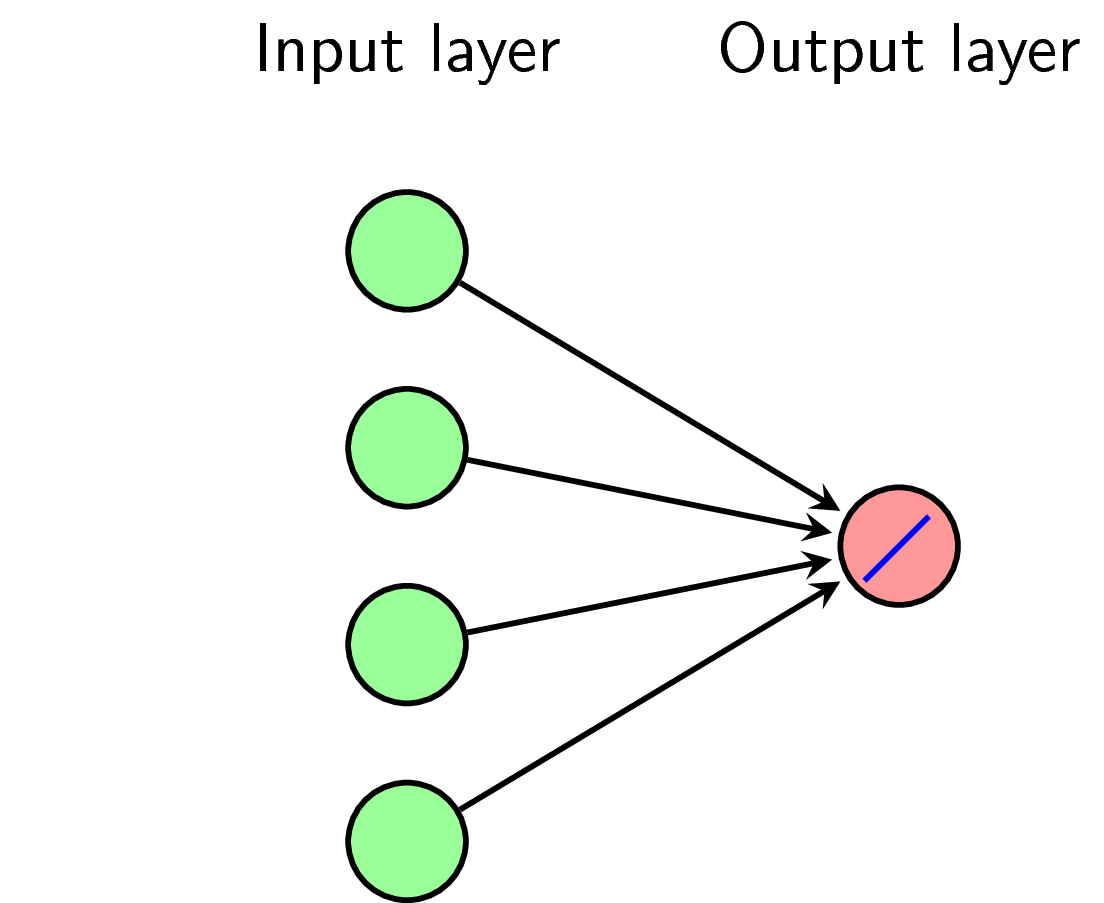
\includegraphics[width=.5\textwidth]{Chapters/05_NeuralNetworks/09_perceptron/lr_nn.png}
    }
\end{figure}

 
Mô hình perceptron ở trên khá giống với một node nhỏ của dây thân kinh sinh học như hình sau đây: 
 
% <div class="imgcap"> 
% <img src ="http://sebastianraschka.com/images/blog/2015/singlelayer_neural_networks_files/perceptron_neuron.png" align = "center" width = "600"> 
% <div class = "thecap">Hình 7: Mô tả một neuron thần kinh sinh học. (Nguồn: <a href = "http://sebastianraschka.com/Articles/2015_singlelayer_neurons.html">Single-Layer Neural Networks and Gradient Descent</a>)</div> 
% </div>  

% \begin{figure}[t]
%     % caption on side     
%     \floatbox[{\capbeside\thisfloatsetup{capbesideposition={right,top},capbesidewidth=6cm}}]{figure}[\FBwidth]
%     {\caption{ 
    
%     }
%     \label{fig:}}
%     { % figure here
%     \includegraphics[width=.5\textwidth]{}
%     }
% \end{figure}

{\color{red} IMG}

 
 
Dữ liệu từ nhiều dây thần kinh đi về một \textit{cell nucleus}. Thông tin được tổng hợp và được đưa ra ở output. Nhiều bộ phận như thế này kết hợp với nhau tạo nên hệ thần kinh sinh học. Chính vì vậy mà có tên Neural Networks trong Machine Learning. Đôi khi mạng này còn được gọi là Artificial Neural Networks (ANN) tức \textit{hệ neuron nhân tạo}.  
 
 
\section{Thảo Luận}
 
\subsection{PLA có thể cho vô số nghiệm khác nhau }
Rõ ràng rằng, nếu hai class là linearly separable thì có vô số đường thằng phân cách 2 class đó (Xem Hình \ref)
 
% <div class="imgcap"> 
% <img src ="/assets/pla/pla6.png" align = "center" width = "400"> 
% <div class = "thecap">Hình 8: PLA có thể cho vô số nghiệm khác nhau.</div> 
% </div>

\begin{figure}[t]
      % caption on side     
      \floatbox[{\capbeside\thisfloatsetup{capbesideposition={right,top},capbesidewidth=6cm}}]{figure}[\FBwidth]
      {\caption{ 
      PLA có thể cho vô số nghiệm khác nhau.
      }
      \label{fig:9_8}}
      { % figure here
      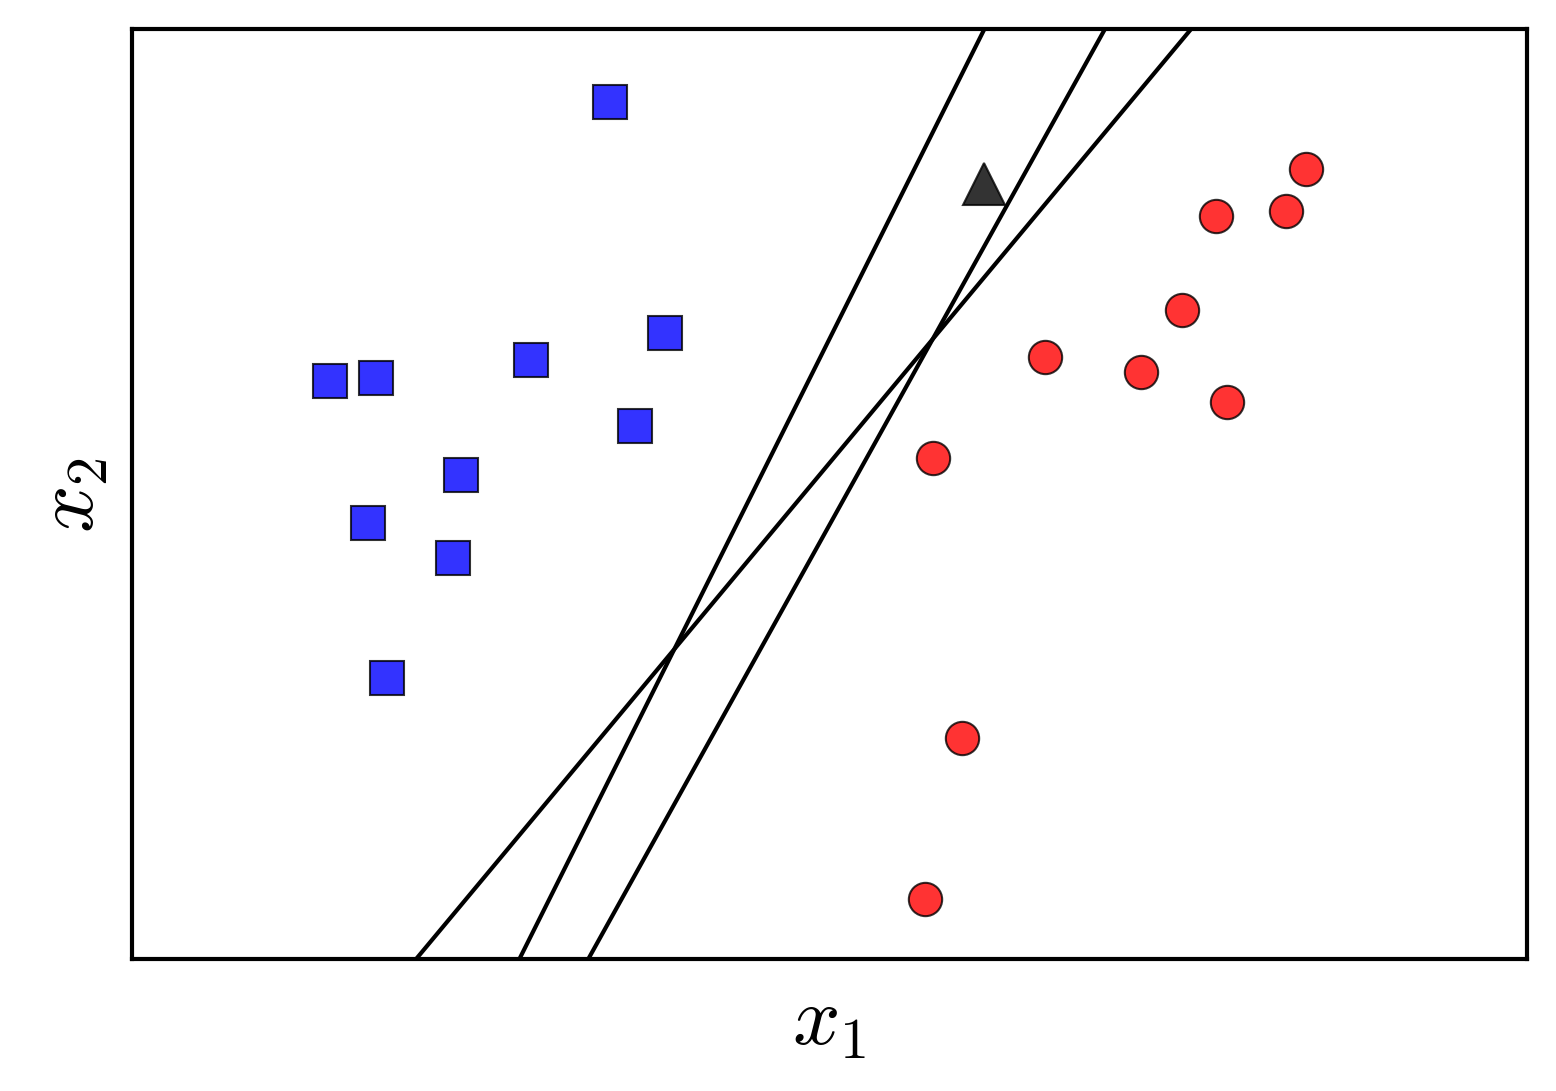
\includegraphics[width=.5\textwidth]{Chapters/05_NeuralNetworks/09_perceptron/pla6.png}
      }
  \end{figure}

 
Tất cả các đường thẳng màu đen đều thỏa mãn. Tuy nhiên, các đường khác nhau sẽ quyết định điểm hình tam giác thuộc các lớp khác nhau. Trong các đường đó, đường nào là tốt nhất? Và định nghĩa "tốt nhất" được hiểu theo nghĩa nào? Có một thuật toán khác định nghĩa và tìm đường tốt nhất như thế, tôi sẽ giới thiệu trong 1 vài bài tới. Mời các bạn đón đọc.  
 
 
\subsection{PLA đòi hỏi dữ liệu linearly separable}
 
Hai class trong ví dụ dưới đây \textit{tương đối} linearly separable. Mỗi class có 1 điểm coi như \textit{nhiễu} nằm trong khu vực các điểm của class kia. PLA sẽ không làm việc trong trường hợp này vì luôn luôn có ít nhất 2 điểm bị misclassified.  
 
% <div class="imgcap"> 
% <img src ="/assets/pla/pla7.png" align = "center" width = "400"> 
% <div class = "thecap">Hinhf 9: PLA không làm việc nếu chỉ có một nhiễu nhỏ.</div> 
% </div> 

\begin{figure}[t]
     % caption on side     
     \floatbox[{\capbeside\thisfloatsetup{capbesideposition={right,top},capbesidewidth=6cm}}]{figure}[\FBwidth]
     {\caption{ 
     PLA không làm việc nếu chỉ có một nhiễu nhỏ.
     }
     \label{fig:9_7}}
     { % figure here
     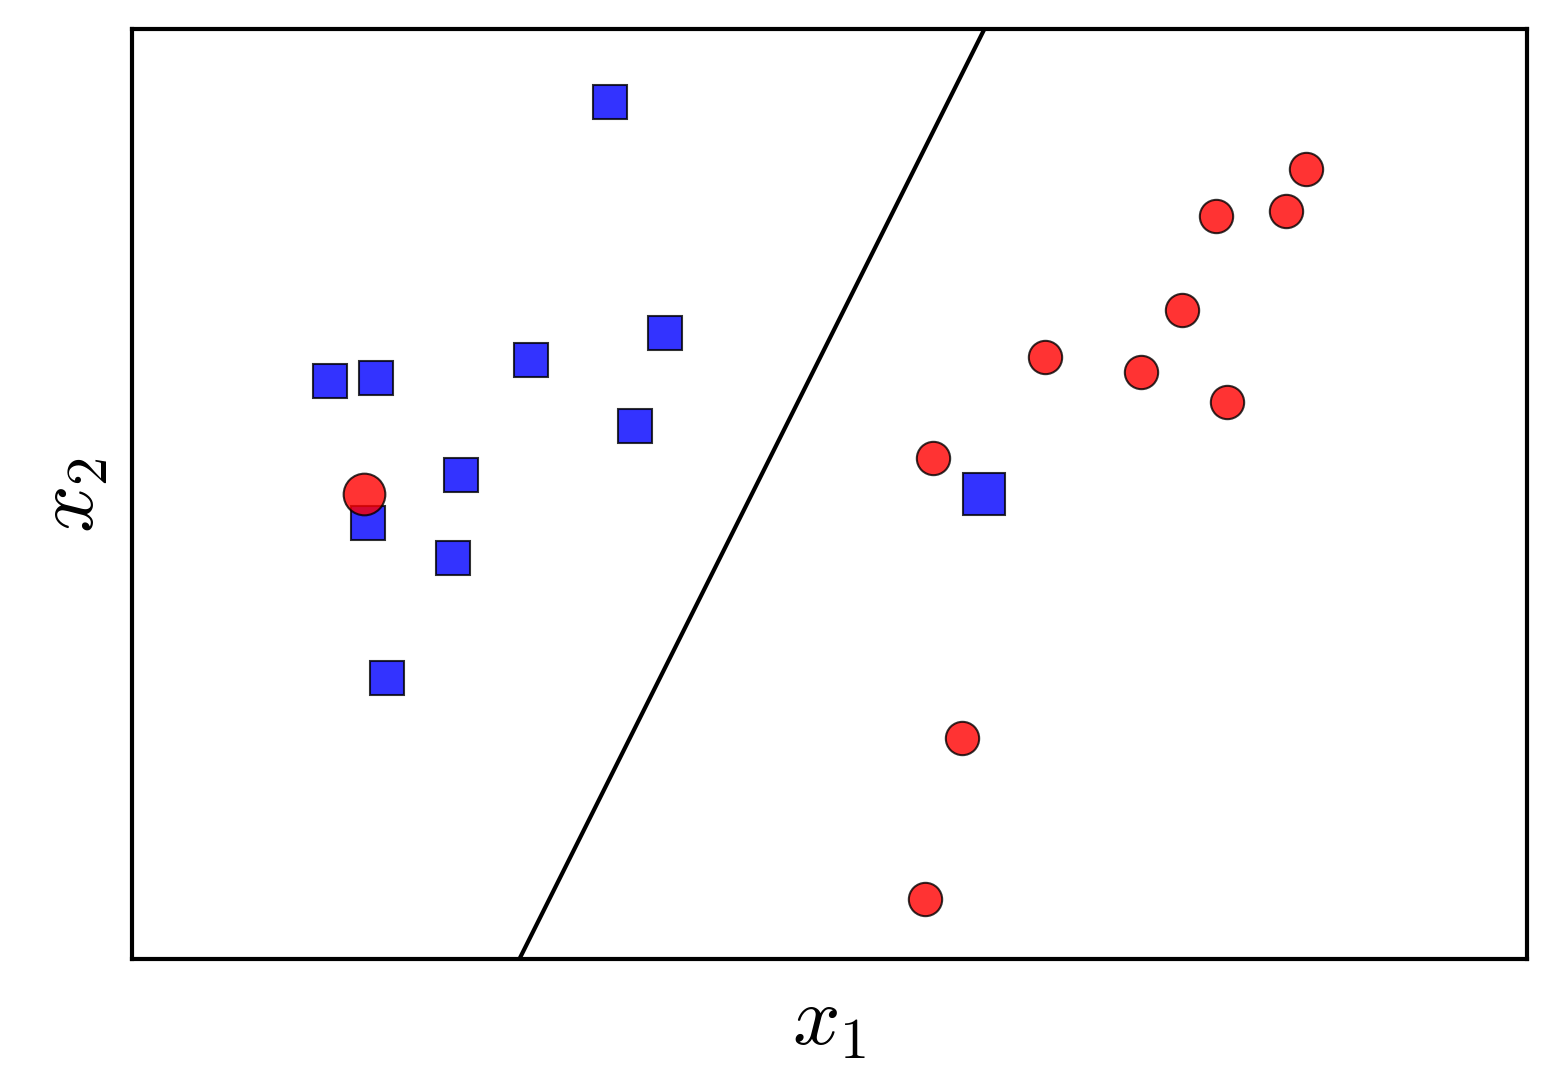
\includegraphics[width=.5\textwidth]{Chapters/05_NeuralNetworks/09_perceptron/pla7.png}
     }
 \end{figure}

 
Trong một chừng mực nào đó, đường thẳng màu đen vẫn có thể coi là một nghiệm tốt vì nó đã giúp phân loại chính xác hầu hết các điểm. Việc không hội tụ với dữ liệu \textit{gần} linearly separable chính là một nhược điểm lớn của PLA. 
 
Để khắc phục nhược điểm này, có một cải tiến nhỏ như thuật toán Pocket Algorithm dưới đây: 
 
\subsection{Pocket Algorithm}
Một cách tự nhiên, nếu có một vài \textit{nhiễu}, ta sẽ đi tìm một đường thẳng phân chia hai class sao cho có ít điểm bị misclassified nhất. Việc này có thể được thực hiện thông qua PLA với một chút thay đổi nhỏ như sau: 

\begin{enumerate}
    \item Giới hạn số lượng vòng lặp của PLA. 

    \item  Mỗi lần cập nhật nghiệm $\mathbf{w}$ mới, ta đếm xem có bao nhiêu điểm bị misclassified. Nếu là lần đầu tiên, giữ lại nghiệm này trong \textit{pocket} (túi quần). Nếu không, so sánh số điểm misclassified này với số điểm misclassified của nghiệm trong \textit{pocket}, nếu nhỏ hơn thì \textit{lôi} nghiệm cũ ra, đặt nghiệm mới này vào.  
\end{enumerate}
 
Thuật toán này giống với thuật toán tìm phần tử nhỏ nhất trong 1 mảng.  
 
 
\section{Kết luận}
 
Hy vọng rằng bài viết này sẽ giúp các bạn phần nào hiểu được một số khái niệm trong Neural Networks. Trong một số bài tiếp theo, tôi sẽ tiếp tục nói về các thuật toán cơ bản khác trong Neural Networks trước khi chuyển sang phần khác.  
 
Trong tương lai, nếu có thể, tôi sẽ viết tiếp về Deep Learning và chúng ta sẽ lại quay lại với Neural Networks. 
 
 
\section{Tài liệu tham khảo}
 
[1] F. Rosenblatt. The perceptron, a perceiving and recognizing automaton Project Para. Cornell Aeronautical Laboratory, 1957. 
 
[2] W. S. McCulloch and W. Pitts. A logical calculus of the ideas immanent in nervous activity. The bulletin of mathematical biophysics, 5(4):115–133, 1943. 
 
[3] B. Widrow et al. Adaptive ”Adaline” neuron using chemical ”memistors”. Number Technical Report 1553-2. Stanford Electron. Labs., Stanford, CA, October 1960. 
 
[3] Abu-Mostafa, Yaser S., Malik Magdon-Ismail, and Hsuan-Tien Lin. Learning from data. Vol. 4. New York, NY, USA:: AMLBook, 2012. (\href{http://work.caltech.edu/telecourse.html}{link to course}) 
 
[4] Bishop, Christopher M. "Pattern recognition and Machine Learning.", Springer  (2006). (\href{http://users.isr.ist.utl.pt/~wurmd/Livros/school/Bishop%20-%20Pattern%20Recognition%20And%20Machine%20Learning%20-%20Springer%20%202006.pdf}{book}) 
 
[5] Duda, Richard O., Peter E. Hart, and David G. Stork. Pattern classification. John Wiley \& Sons, 2012. 
 
